\subsection{\techNew{}}
\label{sec:techc}
% \subsection{Data Locality in Micrographs}
\label{sec:technew}

%基于
\noindent
\zrdnew{
	\textbf{Observation III: }
%	{Important token indices exhibit strong consistency across adjacent layers of an LLM.} To further analyze the distribution of important token indices, we examine the similarity of the top 25\% important token sets across adjacent layers for different models. As shown in Figure~\ref{fig:ob3}(a), there are two key observations: (1) the important tokens exhibit strong consistency across layers, and (2) tokens with higher importance in one layer are more likely to remain important in the subsequent layer.
We summarize two key observations regarding the stability of token importance across layers: 
(1) tokens with higher importance scores in the current layer are  more likely to remain important in the subsequent layer; 
and (2) the probability of a token remaining important in the next layer is positively correlated with its importance score in the current layer. Tokens with higher importance values are more likely to stay important, while those with lower importance values have a decreasing probability of remaining important in the next layer.
To illustrate these observations, 
Figure~\ref{fig:ob3}(a) shows the probability that a token remains important in the next layer. We take the top 25\% tokens with the highest importance values as important tokens. The x-axis represents the top $n$\% of these important tokens ranked by importance, and the y-axis shows the proportion that remain important in the next layer, averaged over 32 layers. Specifically, xxx.
}



%
\begin{figure}
	\centering
	\subfigure[select the top 25\% most important tokens]{
		\includegraphics[width=1.5in, height=1in]{sim-25-cross-layers.pdf}
	}
	\subfigure[select different percentage most important tokens]{
		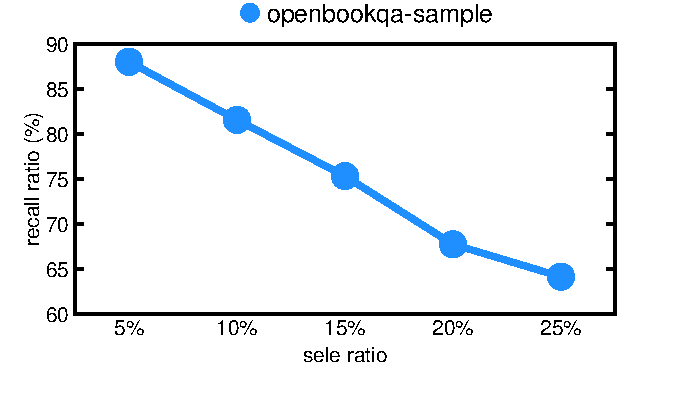
\includegraphics[width=1.5in, height=1in]{recall-sele.pdf}
	}
	\vspace{-0.1in}
	\caption{Similarities of important token index sets of adjacent layers.}
	\label{fig:ob3}
	\vspace{-0.1in}
\end{figure}
%如图xx所示,在模型的一层内,识别重要token index set和加载重要token的kv是有数据依赖的,在没有识别得到重要token index set的情况下,我们无法准确预取下一层所需的重要kv,因此在此层计算时,宝贵的I/O带宽没有被利用,在一个本就I/O瓶颈的场景下。一个naive的方法是,随机的预取一些下一层可能用到的token的kvs到GPU memory中,在下一层的重要token选择完成后,再把不在gpu mem的重要kv load到gpu mem中,然而这样的方法受制于完全不知道下一层重要token index的分布,准确率差,浪费了I/O带宽。一些工作提出了attention sink的概念,即一些特定位置的token在推理过程中总是重要的,如prompt的开头和结尾的几个token,然而,仅预取sink位置的token准确率仍不一定高(一些引用),且存在带宽利用不充分的可能。因此我们提出一种准确率高,灵活的指导预取的方法,高效的预取下一层的重要kv,并将预取与计算overlap起来。我们study了\cref{sec:techa}中提到的识别重要token的方法所识别出的重要token,发现在模型的相邻层重要token的分布是相似的,且重要性排名分位越靠前的index集合,相似度越高。相似度仍用jaccard index量化。
%图片xx描述了基于相似性的重要token识别方法识别出的,图片xx

%\zrdnew{For the important tokens identified as shown in Figure xx, within a given layer of the model, there exists a data dependency between identifying the important token index set and loading the corresponding prefix KVs. Without first identifying the important token index set, we are unable to accurately prefetch the necessary KVs for the next layer. As a result, valuable I/O bandwidth remains underutilized during computation in a scenario that is already constrained by I/O bottlenecks. A naive approach would be to randomly prefetch some potential KVs for the next layer into GPU memory. After the important token selection for the next layer is completed, any important KVs not already in GPU memory can then be loaded into it. However, this approach suffers from the challenge of not knowing the distribution of the important token index set for the next layer, resulting in low accuracy and wasted I/O bandwidth. Some works have proposed the concept of attention sinks, where certain tokens at specific positions, such as the beginning and end of a prompt, are always important during inference. However, prefetching only these sink tokens may still result in low accuracy (some references), and there is a risk of inefficient bandwidth utilization.}
%
%\zrdnew{To address these issues, we propose a more accurate and flexible guidance-based prefetching method that efficiently prefetches important KVs for the next layer while overlapping prefetching with computation. We studied the important tokens identified by the method mentioned in \cref{sec:techa} and found that the distribution of important tokens in adjacent layers is highly similar. Moreover, the index sets with higher importance rankings exhibit higher similarity. This similarity is quantified using the Jaccard index.}

\cp{
\textbf{Design.} 
As shown in Figure~\ref{fig:simiload-ttft}(b), KV loading can only start after token selection completes, creating a dependency that causes GPU stalls and limits computation–I/O overlap.
To mitigate this overhead, we employ prefetching to overlap data loading with computation. 
However, a key challenge remains: the important tokens for the next transformer layer cannot be identified until the current layer’s computation completes, making it difficult to determine which KVs to prefetch in advance.}

\cp{To solve this challenge, based on \textit{Observation~III}, we propose the \technew{} mechanism, which exploits the strong similarity of important token index sets across adjacent layers. 
During the computation of the current layer, \technew{} asynchronously prefetches the next layer’s important KVs into GPU memory by leveraging the importance distribution from the current layer. 
For example, 
as illustrated in Figure~\ref{fig:simiload-ttft}(b), KV loading in Layer~1 cannot begin until token selection completes, causing GPU stalls. 
In contrast, Figure~\ref{fig:simiload-ttft}(c) shows that using Layer~0’s importance information to guide the prefetching of Layer~1’s KVs during computation effectively hides I/O latency and reduces idle time. 
Specifically, the important token positions identified in Layer~0 are used as an approximation of those in Layer~1, allowing the system to prefetch the corresponding key–value pairs of tokens at the same positions in the next layer, making them readily available when computation proceeds.
}


\cp{
While \technew{} effectively hides part of the I/O latency, efficient prefetching still faces two key challenges. 
First, approximating the next layer’s important tokens using those of the current layer can leave a portion of the selections inaccurate, so improving prefetch accuracy and providing a recovery mechanism to fetch missing data are both essential.
Second, the prefetching I/O must be carefully coordinated with computation. 
If computation takes longer than prefetching, the I/O bandwidth remains underutilized; conversely, if prefetching exceeds computation time, speculative I/O lies on the critical path, and any mispredicted prefetches can introduce additional latency.}


\cp{
To tackle the first issue, based on \textit{Observation~III}, we rank all candidate tokens by their importance scores in the current layer and prefetch their corresponding KVs in descending order, as tokens with higher importance are more likely to remain important at the same indices in the next layer. 
Before the next layer begins computation, a probe \textit{head-K} loading operation validates the prefetched results and synchronously loads any missing KVs on the critical path, as shown by the red-bordered KV loading in Figure~\ref{fig:simiload-ttft}(c).}


\cp{
To address the second issue, it is essential to ensure that computation and prefetching I/O are well aligned in time. 
Achieving this requires accurate estimation of both computation and I/O durations. 
For computation, we observe that during the prefill stage of inference, the workload across transformer layers remains roughly constant, as their structural design is identical.
Therefore, we use the measured computation time of the first layer as an estimate for all subsequent layers, which serves as the time budget for prefetching. }

\cp{
For I/O estimation, K and V vectors are stored in fixed-size chunks, each containing multiple token entries (e.g., \texttt{chunksize}=64). 
Given a set of target token IDs, we map each token to its chunk and determine the storage tier. 
Chunks on SSD are first mmap-loaded into CPU memory before the required K/Vs are transferred to GPU via PCIe, while chunks in CPU memory are directly transferred and GPU-resident chunks are accessed immediately. 
Profiling shows that chunk-fetch latency within each tier is stable and predictable. 
Therefore, we profile the average per-chunk latency across different storage tiers (SSD, CPU, GPU) by measuring multiple fetch operations on each medium and taking their mean values as reference. 
Using these profiled averages, we load chunks in descending order of token importance until the prefetching window is filled. 
This ensures that prefetching time closely matches computation, effectively hiding I/O latency behind GPU execution.}




%\cp{A straightforward approach is to prefetch data in descending order of importance scores from the previous layer. However, this strategy introduces two major issues.
%(1) The predicted importance is not always accurate (in Figure~\ref{}). Incorrectly prefetched data from SSD can waste substantial parallel I/O time, so the amount of SSD-prefetched data must be carefully controlled.
%(2) Another challenge arises when not all required data are successfully prefetched before inference, leading to missing inputs during computation and requiring a remedy mechanism.}
%
%\cp{
%To mitigate the first issue, we design a dual-tier prefetching (DTP) mechanism that controls the proportion of data fetched from different storage tiers.
%Let $T_{\text{comp}}$ be the computation window during which data loading overlaps with GPU computation.
%DTP divides this window by a ratio $\delta$: $\delta T_{\text{comp}}$ is allocated for memory loading and $(1-\delta)T_{\text{comp}}$ for SSD loading.
%Within each tier, tokens are sorted by predicted importance and prefetched in descending order until the respective budget is used up.
%This confines SSD reads while maintaining effective overlap between I/O and computation.
%Extensive experiments across various workloads show that $\delta=0.8$ consistently achieves the best inference efficiency, as shown in Figure~\ref{}. 
%Thus, \pname{} uses a fixed $\delta=0.8$ in all experiments, while adaptive tuning is left for future work.
%}
%
%\cp{
%To ensure all required data are available during inference, we introduce a lightweight recovery mechanism. After each prefetching window, the system performs a Head-\(K\) loading operation for the next layer to validate prefetched results and fetch missing important KVs, as shown by the red-bordered KV loading in Figure~\ref{fig:simiload-ttft}(c). Token selection is also performed at each layer to update the importance distribution based on the latest computation, ensuring that subsequent prefetching remains accurate. Additionally, incorrectly prefetched data are retained and reused during inference to avoid unnecessary I/O waste.
%}

